\documentclass[fleqn]{article}
\usepackage[english]{babel}
\usepackage{amsmath}
\usepackage{amsthm}
\usepackage{graphicx}
\usepackage[utf8]{inputenc}

%%%%%%%% MARGIN
\usepackage[left=1in, right=1in, top=0.8in, bottom=0.8in]{geometry}

%%%%%%%% NO PARAGRAPH INDENT
% https://tex.stackexchange.com/questions/27802/set-noindent-for-entire-file
\setlength\parindent{0pt}

%%%%%%%% SUB-FIGURE PACKAGE
\usepackage{subcaption}

\usepackage{pdfpages}

%%%%%%%% HYPERREF PACKAGE
\usepackage{hyperref}
\hypersetup{linkcolor=blue}
\hypersetup{citecolor=blue}
\hypersetup{urlcolor=blue}
\hypersetup{colorlinks=true}

%%%%%%%% MULTI-COLUMNS PACKAGE
\usepackage{multicol}

%%%%%%%% SETS DEFINITIONS
\usepackage{amssymb}
%%%% Important sets
\renewcommand{\O}{\mathbb{O}}
\newcommand{\N}{\mathbb{N}}
\newcommand{\Z}{{\mathbb{Z}}}
\newcommand{\Q}{{\mathbb{Q}}}
\newcommand{\R}{{\mathbb{R}}}

%%%% Statistics
\newcommand{\E}[1]{\mathbb{E}\left[#1 \right]}
\newcommand{\V}[1]{\mathbb{V}\left[#1 \right]}
\newcommand{\cov}[1]{\mathrm{Cov}\left[#1 \right]}

%%% Misc Math
% Spaces after/before left/right
\let\originalleft\left
\let\originalright\right
\renewcommand{\left}{\mathopen{}\mathclose\bgroup\originalleft}
\renewcommand{\right}{\aftergroup\egroup\originalright}

% Norm
\newcommand{\norm}[1]{\left\lVert#1\right\rVert}

%%%% Superscript to the left
% https://latex.org/forum/viewtopic.php?t=455
\usepackage{tensor}
\newcommand{\app}[3]{\tensor*[^{#1}]{\left(#2, #3\right)}{}}


%%%%%%%% SPLIT EQUATIONS
% https://tex.stackexchange.com/questions/51682/is-it-possible-to-pagebreak-aligned-equations
\allowdisplaybreaks

%%%%%%%% CODE RENDERING
% Compile with flag -shell-escape
\usepackage{minted}

%%%%%%%% EXAM PACKAGE
\usepackage{mathexam}

%%%%%%%% CHANGE MARGINS ITEMIZE
\usepackage{enumitem}

%%%%%%%% START DOCUMENT

\ExamClass{EC0301 - Time Series}
\ExamName{Assignment \#2}
\ExamHead{\today}

\let\ds\displaystyle

\begin{document}
 \vspace{0.3cm}
   % Information of the student
   \begin{itemize}[leftmargin=6.25cm, labelsep=0.5cm]

     \item[\textit{Name}] \scalebox{1.2}{David Plazas Escudero} % Name
     \item[\textit{Student code}] 201710005101 % Code

   \end{itemize}
\vspace{0.3cm}

% Each of the items to solve
\begin{enumerate}
\item \textit{Consider an AR(2) model. Prove that the following conditions must be satisfied for $\lambda_1$ and $\lambda_2$ to be inside the unit circle: i) $\phi_1+\phi_2<1$, ii) $-\phi_1+\phi_2<1$ and $|\phi_2|<1$.}

Recall that the solutions $\lambda_{1,2}$ are solutions to 
\[
\lambda^2 - \phi_1\lambda - \phi_2=0
\]
and then, they can be explicitly calculated as
\[
\lambda_{1,2} = \dfrac{\phi_1\pm\sqrt{\phi_1^2+4\phi_2}}{2}.
\]
This solutions can be classified in two cases: $\phi_1^2+4\phi_2\geq0$ and $\phi_1^2+4\phi_2<0$. Let us assume first that $\phi_1^2+4\phi_2\geq0$ and, therefore, $\lambda_i\in\mathbb{R}$. As these roots are real, they lie inside the unit circle whenever $|\lambda_i|<1$. Hence,
\[
\left|\dfrac{\phi_1\pm\sqrt{\phi_1^2+4\phi_2}}{2}\right|<1\implies
-2<\phi_1\pm\sqrt{\phi_1^2+4\phi_2}<2.
\]
Let us work with the right-most inequality:
\[
\begin{split}
\phi_1\pm\sqrt{\phi_1^2+4\phi_2}&<2\\
\sqrt{\phi_1^2+4\phi_2}&<2\mp\phi_1\\
\phi_1^2+4\phi_2&<4\mp 4\phi_1+\phi_1^2\\
\phi_2&<1\mp\phi_1
\end{split}
\]
and from this last result we can directly obtain conditions i) and ii). 

Now, let us assume that $\phi_1^2+4\phi_2<0$ and, thus, $\lambda_i\in\mathbb{C}$. Given the complex nature of the roots, they will lie inside the unit circle whenever $\norm{\lambda_i}<1$, where $\norm{\cdot}$ is the standard euclidean norm in the $\mathbb{C}$ normed vector space.

Recall that 
\[
\lambda_{1,2} = \dfrac{\phi_1\pm\sqrt{\phi_1^2+4\phi_2}}{2}.
\]
As $\phi_1^2+4\phi_2<0$, the above expression can be rewritten as
\[
\lambda_{1,2} = \dfrac{\phi_1}{2}\pm\dfrac{\sqrt{-(\phi_1^2+4\phi_2})}{2}i,
\]
where $i=\sqrt{-1}$ is the imaginary unit. Thus,
\[
\norm{\lambda_i}^2=\dfrac{\phi_1^2}{4}+\dfrac{-(\phi_1^2+4\phi_2)}{4}=-\phi_2,
\]
and then $-\phi_2<1$ or $\phi_2>-1$, which is equivalent to $|\phi_2|<1$ and, therefore, condition iii) is proved.

\item \textit{Find the parameters $\phi_1$ and $\phi_2$ of an AR(2) with autocorrelations $\rho_1=0.8$ and $\rho_2=0.6$.}

The parameters for the AR(2) model can be found by the Yule-Walker's system of equations
\[
\begin{bmatrix}
\phi_1\\\phi_2
\end{bmatrix} = \begin{bmatrix}1 & \rho_1\\\rho_1 & 1\end{bmatrix}^{-1}\begin{bmatrix}
\rho_1 \\ \rho_2
\end{bmatrix}.
\]
In our case,
\[
\begin{bmatrix}
\phi_1\\\phi_2
\end{bmatrix} = \begin{bmatrix}1 & 0.8\\0.8 & 1\end{bmatrix}^{-1}\begin{bmatrix}
0.8 \\ 0.6
\end{bmatrix}=\begin{bmatrix}1 & 4/5\\4/5 & 1\end{bmatrix}^{-1}\begin{bmatrix}
4/5 \\ 3/5
\end{bmatrix}=\dfrac{25}{9}\begin{bmatrix}1 & -4/5\\-4/5 & 1\end{bmatrix}\begin{bmatrix}
4/5 \\ 3/5
\end{bmatrix}=\dfrac{1}{45}\begin{bmatrix}100-60\\-80+75\end{bmatrix}=\begin{bmatrix}8/9\\-1/9\end{bmatrix}.
\]

\item Simulate 1000 observations of the two following AR(2) models: i) $x_t=-0.8x_{t-1}+0.4x_{t-2}+\varepsilon_t$ and ii) $x_t=0.6x_{t-1}-0.9x_{t-2}+\varepsilon_t$ and show the autocorrelation plot. What can be concluded from the form these autocorrelation plots?

Let us first show the code to simulate an AR(2) model:
\begin{minted}{python}
import numpy as np
import pandas as pd
import scipy.stats as st
import matplotlib.pyplot as plt

plt.rc('text', usetex=True)
plt.rcParams.update({'font.size': 15})

# Global Parameters
sigma2 = 2
mu = 0
T = 1000
x0 = (0,0)

def ar2(mu, phi1, phi2, T, x0):
    e = st.norm.rvs(size=(T), loc=0, scale=sigma2**0.5)
    xs = np.zeros(T)
    xs[0:2] = x0
    for i in range(2, len(xs)):
        xs[i] = mu + phi1 * xs[i-1] + phi2 * xs[i-2] + e[i]
    return xs
\end{minted}

For model i), the specific simulation and plot code is
\begin{minted}{python}
# Specific Parameters
phi11 = -0.8
phi21 = 0.4

# Simulation
xs1 = ar2(mu, phi11, phi21, T, x0)

# Autocorrelation plot and figure export
ax1 = pd.plotting.autocorrelation_plot(xs1[:50])
ax1.set_title('$x_{t}=-0.8x_{t-1}+0.4x_{t-2}+\epsilon_t$')
plt.savefig('TS1.pdf', bbox_inches='tight')
\end{minted}

The obtained autocorrelation plot is presented in Fig. \ref{fig:ts1}. Note that this autocorrelation plot only is presented for 50 lags; this is due to the fast decrease on the correlation as the lags increase. After 50 lags, the correlation is negligible and, thus, it is not presented in this figure. It can be observed that this autocorrelation oscillates around the lag axis and after 7 lags, all the autocorrelations lie inside the confidence bands.

Furthermore, this model does not satisfy the three conditions for stationarity of an AR(2) model; specifically, condition ii) is not met since $-\phi_1+\phi_2=0.8+0.4=1.2>1$.


\begin{figure}[H]
    \centering
    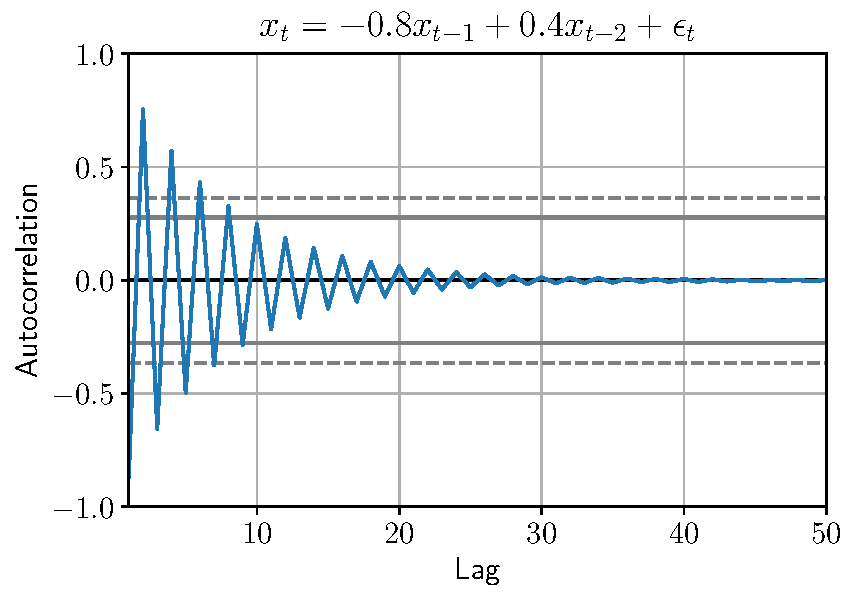
\includegraphics[scale=.6]{figs/TS1.pdf}
    \caption{Autocorrelation plot for model i).}
    \label{fig:ts1}
\end{figure}

For model ii), the specific simulation and plot code is
\begin{minted}{python}
# Specific Parameters
phi12 = 0.6
phi22 = -0.9

# Simulation
xs2 = ar2(mu, phi12, phi22, T, x0)

# Autocorrelation plot and figure export
ax2 = pd.plotting.autocorrelation_plot(xs2)
ax2.set_title('$x_{t}=0.6x_{t-1}-0.9x_{t-2}+\epsilon_t$')
plt.savefig('TS2.pdf', bbox_inches='tight')
\end{minted}

The obtained autocorrelation plot is presented in Fig. \ref{fig:ts2}. Unlike the plot for model i), this figure shows the autocorrelation for all lags since, as it can observed, it shows an important behavior along the complete set of lags. It can be observed that the magnitude of the autocorrelation is decreasing as the lags increase, although it appears to be significant again between lags 350 and 500. Note that this model does satisfy all three conditions for stationarity.

\begin{figure}[H]
    \centering
    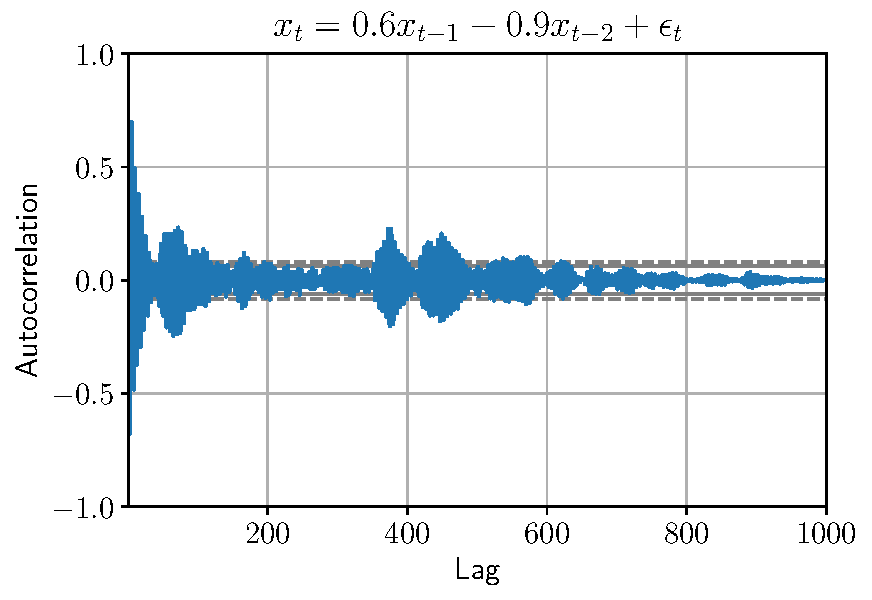
\includegraphics[scale=.6]{figs/TS2.pdf}
    \caption{Autocorrelation plot for model ii).}
    \label{fig:ts2}
\end{figure}

\end{enumerate}
\end{document}
